\documentclass[tikz,border=10pt]{standalone}
\usepackage{amsmath}
\usepackage{tikz}
\usetikzlibrary{arrows.meta,calc,positioning}

\tikzset{
  signal/.style={->, line width=1.2pt, draw=black!80, >=Stealth},
  block/.style={draw=blue!70!black, line width=1.2pt, rectangle, rounded corners=2pt, minimum width=2.8cm, minimum height=1.0cm, align=center, fill=none},
  note/.style={font=\small, align=center}
}

\begin{document}
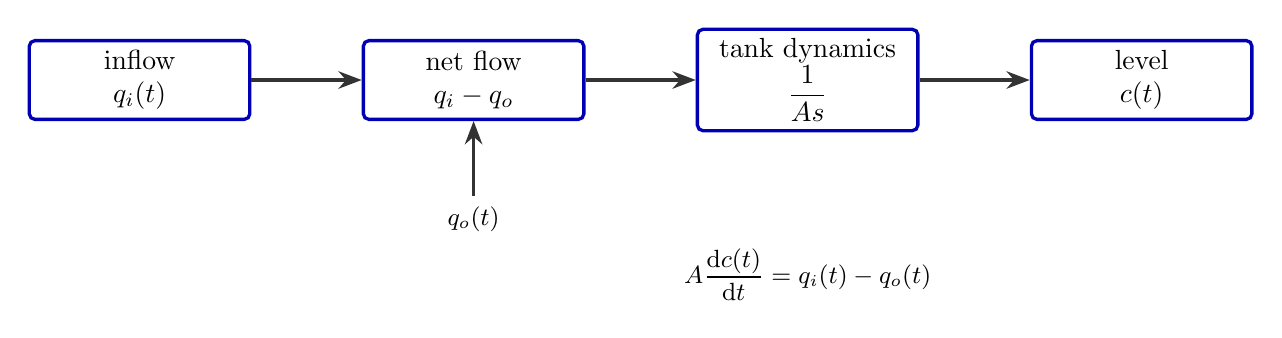
\begin{tikzpicture}[node distance=1.4cm]
  \node[block] (qin) {inflow\\$q_i(t)$};
  \node[block, right=of qin] (sum) {net flow\\$q_i-q_o$};
  \node[block, right=of sum] (tank) {tank dynamics\\$\dfrac{1}{A s}$};
  \node[block, right=of tank] (level) {level\\$c(t)$};
  \draw[signal] (qin) -- (sum);
  \draw[signal] (sum) -- (tank);
  \draw[signal] (tank) -- (level);
  \draw[signal] ($(sum.south)+(0,-0.15)$) -- ++(0,-0.8) -| node[pos=0.25, below, font=\small] {$q_o(t)$} (sum.south);
  \node[note, below=1.35cm of tank] {$A\dfrac{\mathrm{d}c(t)}{\mathrm{d}t}=q_i(t)-q_o(t)$};
\end{tikzpicture}
\end{document}
